
\section{Introduction}
The Risk Modeller's Toolkit (or RMTK) is a Python 2.7 library of functions written by scientists at the GEM Model Facility, which is intended to provide scientists and engineers with the tools to help create the vulnerability input models that go into the OpenQuake risk engine. The intention of this software is to provide scientists and engineers with the means to apply some of the most commonly used algorithms for preparing vulnerability models using structural analysis data. The current approach consists of the derivation of fragility curves and the combination with a damage-to-loss function for the definition of a discrete vulnerability function. The just released GEM analytical vulnerability guidelines have been integrated in this tool and some of the methodologies indicated have been already implemented in the library. In forthcoming versions will hope to make available more methodologies for the process indicated here, and to integrate new functionalities for i) building structural models of different levels of complexity within the RMTK in combination with a structural analysis software, ii) running dynamic and static analysis within the RMTK in combination with a structural analysis software, iii) deriving vulnerability curves directly applying engineering demand parameters-to-loss functions to structural analysis results.

This section provides a description of the methods currently implemented in the RMTK, and an initial presentation of the input and output files is provided. In the following sections, the contents and structure of these files are discussed in detail.

\section{Getting Started and Running the Software}
Install notebook and dependencies
go to folder in the command line (RMTK/Vulnerability/name-of-the-procedure)
 
\section{Nonlinear Static Method with dispersion information}
Nonlinear Static Methods are based on the use of capacity curves resulting from nonlinear static pushover analysis to determine the median seismic intensity values $\hat{s}_c$ corresponding to the attainment of each damage state threshold and the corresponding dispersion $\beta_{sc}$, to represent a fragility curve as the probability of the limit state capacity C being exceeded by the demand D, both expressed in terms of intensity levels (s$_c$ and s respectively).

\begin{equation}
P_{LS}(s) = P(C < D | s) = \Phi(\frac{ln s -ln \hat{s}_c}{\beta_{sc}})
\end{equation}

The methodology implemented so far allows to consider different shapes of the pushover curve, multilinear and bilinear, and record to record dispersion together with dispersion in the damage state thresholds. Different input types can be inserted depending on whether the user has already at his disposal an idealised pushover curve or it has to be derived from the raw results of a pushover analysis. Ruiz-Garcia and Miranda (2007) study on inelastic displacement demand estimation, and Vamvatsikos and Cornell (2006) work on seismic demand estimation with multilinear static pushover curves have been integrated in two nonlinear static procedures, to give the user the chance to select the procedure with the degree of accuracy consistent with the input available and the structural analyses performed. In the following section the two procedures will be presented from the perspective of their implementation in a python script and the necessary scientific background behind it.

\subsection{C$_R$ based procedure}

The C$_R$ based procedure presented herein is applicable to bilinear elasto-plastic capacity curve only. The intensity measure to be used is S$_a$ and a mapping between any engineering demand parameter (EDP), assumed to describe the damage state thresholds, and the roof displacement is available from the pushover analysis. This procedure provides a simple relationship between median damage state threshold, expressed in terms of top displacement $\delta_{roof}$ as previously explained, at each damage state threshold ds and the corresponding median elastic Spectral displacement value $\hat{S}_{d,ds}(T_1)$.

\begin{equation}
\hat{\delta}_{roof, ds} = C_R S_d(T_1) \Gamma_1 \phi_1
\end{equation}

where $\Gamma_1 \Phi_1$ is the first mode participation factor, estimated for the first-mode shape normalised by the roof displacement and C$_R$ is the inelastic displacement ratio (inelastic over elastic spectral displacement), computed by Ruiz-Garcia and Miranda (2007) for nonlinear SDoF systems having hysteretic behaviour representative of the analysed structure, which is a function of the first-mode period of vibration and the relative lateral strength of the system, R. Therefore the median Spectral acceleration at the fundamental period of vibration $\hat{S}_{a,ds}(T_1)$, the seismic intensity measure used in this procedure, turns out to be expressed as a function of the roof displacement according to the following equation:

\begin{equation}
\hat{S}_{a,ds}(T_1) = \frac{4 \pi^2}{C_R T^2 \Gamma_1 \phi_1} \hat{\delta}_{roof, ds}
\end{equation}

Default values of $\hat{C}_R$ parameter estimates are provided by Ruiz-Garcia and Miranda (2007) as result of nonlinear regression analysis of three different measures of central tendency computed from 240 ground motions:

\begin{equation}
\hat{C}_R = 1 + \frac{R - 1}{79.12 T_1 ^{1.98}}
\end{equation}

and values for R are given as:

\begin{equation}
R_ds = max(0.425(1 - c + \sqrt{c^2 + 2c(2 \mu_{ds} - 1) + 1}),1)
\end{equation}

where c = 79.12 T$^{1.98}$, and $\mu_{ds}$ is the ductility at the damage state threshold of interest.

The dispersion of $\hat{S}_{a,ds}(T_1)$ is computed making use of the following relationship with the median EDP damage threshold $\hat{\theta}$ (Cornell, 2002):

\begin{equation}
\hat{\theta}(s) = a s^b
\end{equation}

so that:

\begin{equation}
\beta_{sc} = \frac{1}{b} \beta_{\theta d}
\end{equation}

and if the uncertainty in the damage state threshold $\beta_{\theta c}$ wants to be introduced it can be easily combined with the record-to-record variability in the following equation:

\begin{equation}
\beta_{sc} = \frac{1}{b} \sqrt{\beta_{\theta d}^2 + \beta_{\theta c}^2} 
\end{equation}

Finally the dispersion of $d_{roof}$ is the same as the dispersion of C$_R$, since they are proportional. Asssuming that $d_{roof}$ and the EDP damage threshold are also proportional, they share the same dispersion. Ruiz-Garcia and Miranda (2007) estimated the dispersion of C$_R$ as:

\begin{equation}
\sigma_{\ln(C_R)} = \sigma_{\ln(d_{roof})} = \beta_{\theta d} =  1.975 [\frac{1}{5.876} + \frac{1}{11.749 (T + 0.1)}] [1- \exp(-0.739 (R - 1))]
\end{equation}

\subsubsection{Calculation Steps}
\label{subsec:CalculationSteps}
The medians capacity and corresponding dispersions for different damage thresholds are obtained through the following steps:

\begin{enumerate}
\item Define the inputs: dynamic properties of the building (elastic period and modal participation factor), limit states and pushover curve results.
\item Idealise the pushover curve if the input data consists of a complete not-idealised pushover curve. The only parameters needed to describe the idealised pushover curve are the yielding displacemet $\delta_y$, the ultimate displacement $\delta_u$ and the yielding force F$_y$.
\item Transform the MDoF system to an equivalent SDoF system, and derive the equivalent SDoF-based idealised capacity curve.
\item Define the ductility levels $\mu_{ds}$ corresponding to each damage threshold, expressed in terms of roof displacement.
\item Compute R and C$_r$, using equation (1.5) and (1.4) respectively.
\item Compute $\hat{S}_{a,ds}(T_1)$ and the corresponding dispersion  $\beta_{\theta d}$ using eq. (1.3) and (1.9) respectively.
\item Combine $\beta_{\theta d}$ with dispersion due to uncertainty in the model $\beta_{\theta c}$, if different from zero, using eq. (1.8) to get the total dispersion $\beta_{sc}$.
\end{enumerate}

\subsubsection{Step-by-step procedure}
To get started with this procedure use a command line text editor to enter manually the folder location where the RMTK have been saved. Add the path /RMTK/Vulnerability/NSP, where the Nonlinear Static Method with dispersion information script (NSM\_dispersion.py) is located, as shown in the example below

\begin{Verbatim}[frame=single, commandchars=\\\{\}, samepage=true]
\$ cd path/to/rmtk/folder/Vulnerability/NSP
\end{Verbatim}

From the text editor open iPython browser page with the following command line. 

\begin{Verbatim}[frame=single, commandchars=\\\{\}, samepage=true]
\$ python-2.7 notebook --pylab=inline
\end{Verbatim}

Once the iPython page is opened on your browser, you could find the python scripts contained in the NSP directory (Figure \ref{fig:notebook}). Select the file NSM\_dispersion.ipynb.

\begin{figure}[H]
\centering
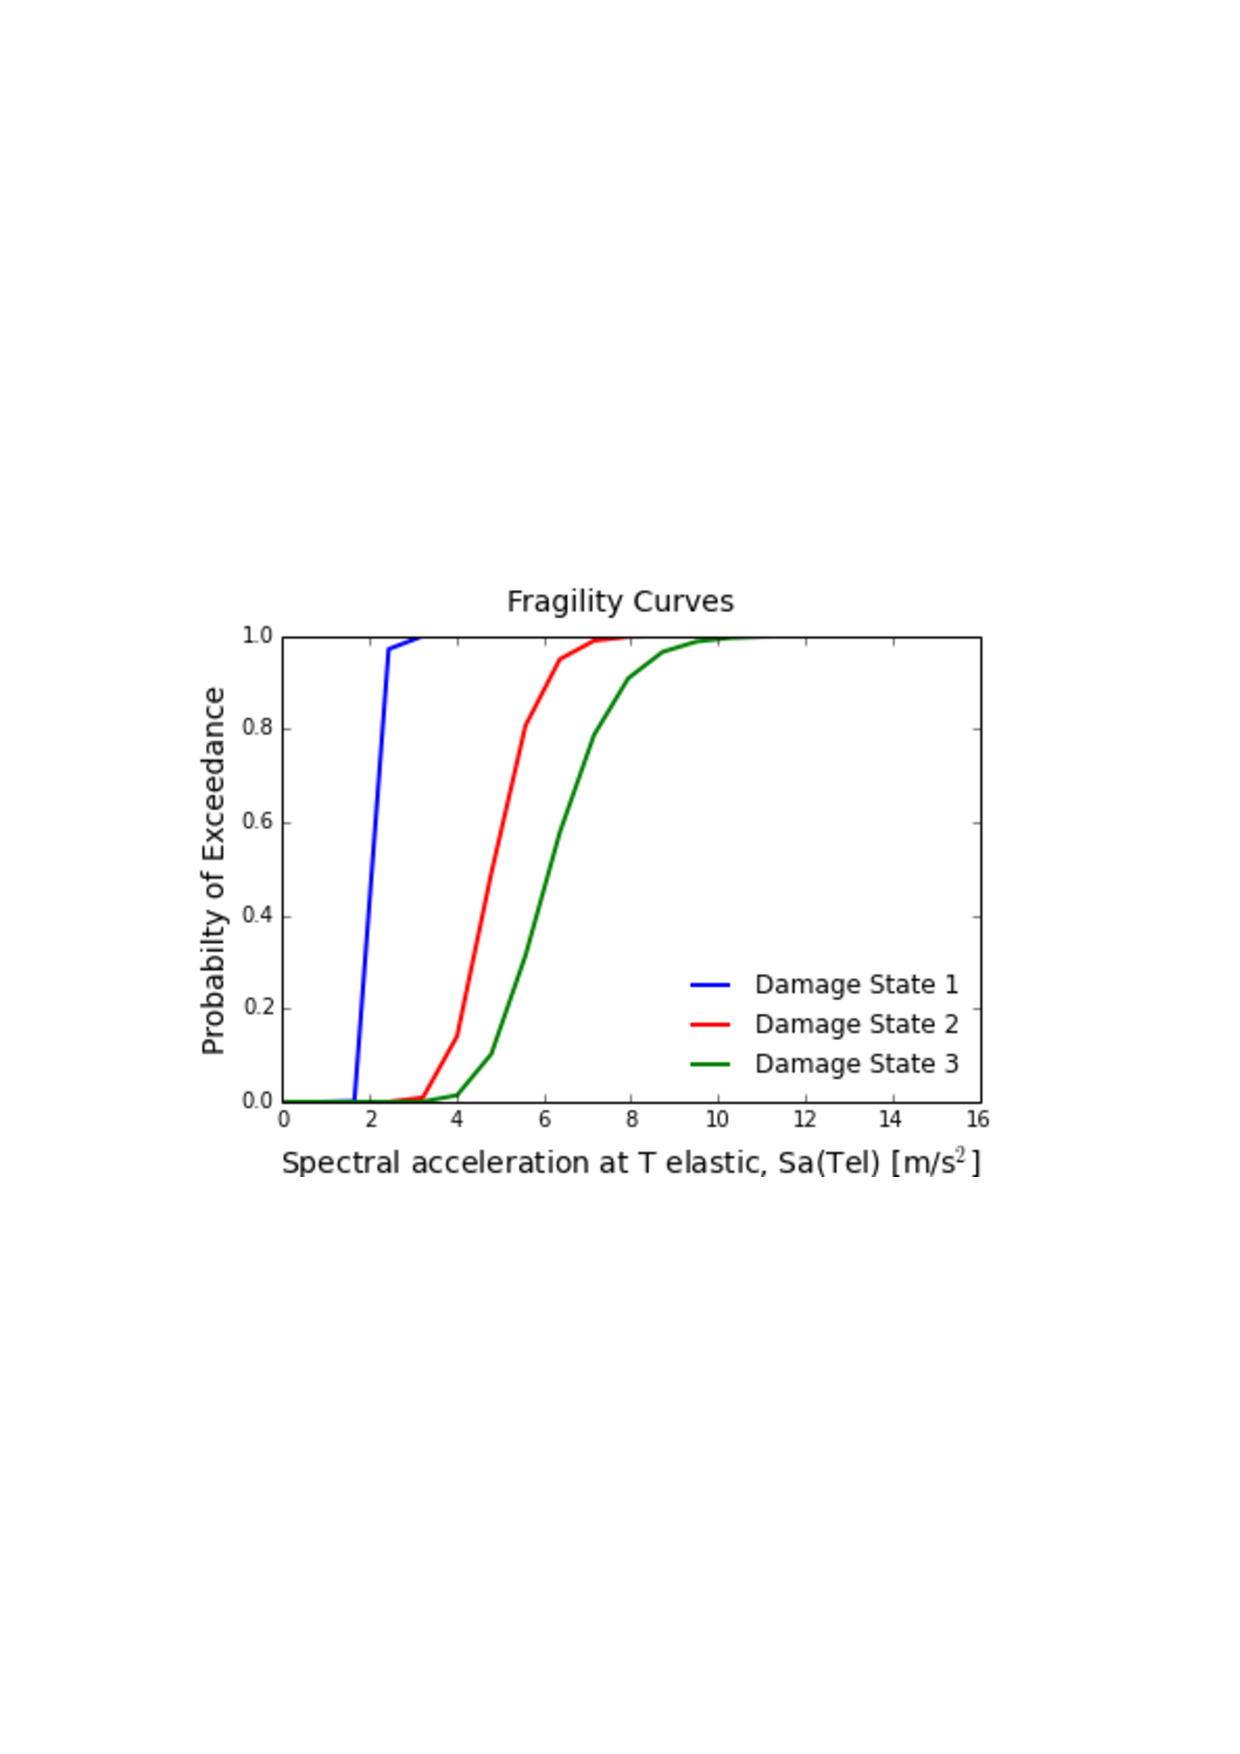
\includegraphics[width=12cm,height=8cm]{./figures/IdealisedCurve.pdf}
\caption{iPython Notebook}
\label{fig:notebook}
\end{figure}

In the first step of the code the initial options and the inputs must be defined, as described in the following section. 

\paragraph{Options}
\label{par:options}
In the Options the user has to define first of all the type of analysis and he wants to perform and the type of inputs he has at his disposal. With the variable an\_type he can choose between:

\begin{Verbatim}[frame=single, commandchars=\\\{\}, samepage=true]
an\_type = 0 # Cr based procedure
an\_type = 1 # spo2ida procedure
\end{Verbatim}

and with the variable in\_type he can choose between:

\begin{Verbatim}[frame=single, commandchars=\\\{\}, samepage=true]
in\_type = 0 # idealised pushover curve
in\_type = 1 # raw results from a pushover analysis
\end{Verbatim}

The variable vulnerability instead gives the opportunity to stop the process at the derivation of the fragility curves, or to go all the way up to the vulnerability curve definition applying damage-to-loss functions.

\begin{Verbatim}[frame=single, commandchars=\\\{\}, samepage=true]
vulnerability = 0 # stop at fragility curves 
vulnerability = 1 # derive vulnerability curve
\end{Verbatim}

The variable g should be a floating number assigned to the gravity acceleration, compatible with the units used for the period of vibration and for displacements (if the period is expressed in seconds and displacements are in meters, then g = 9.81). The variable iml is a numpy array that identifies the intensity measure levels for which loss ratios are computed and provided in the vulnerability curve.

\begin{Verbatim}[frame=single, commandchars=\\\{\}, samepage=true]
g = 9.81
iml = np.linspace(0.1,15,100)
\end{Verbatim}

The variable plotflag allows or inhibits the displaying of plots. It is a list composed of 4 integers, each one controlling a different plot: idealised pushover curve, 16\%-50\%-84\% ida curves, fragility curves, vulnerability curve. Each integer can take value zero or one whether the corresponding graph is to be displayed or not:

\begin{Verbatim}[frame=single, commandchars=\\\{\}, samepage=true]
plotflag = [1, 1, 1, 1] # plot all the graphs
plotflag = [0, 0, 0, 0] # do not plot any graph
\end{Verbatim}

The following variables set some of the characteristics of the plots:

\begin{itemize}
\item linew: integer for defining lines width.
\item fontsize : fontsize used for labels, graphs etc.
\item units: list of 3 strings defining displacements, forces and Spectral acceleration units, as ['[kN]' '[m]' ['m/s\^2]], to be displayed on the axes of the plots
\end{itemize}

The last set of variables is needed for spo2ida procedure:

\begin{itemize}
\item pw: floating number assigning pinching level (from 0 to 1)
\item filletstyle: integer enabling or not the use of a spline line to link branches of IDA curves

\begin{Verbatim}[frame=single, commandchars=\\\{\}, samepage=true]
filletstyle = 0 # don't use spline curve
filletstyle = 3 # use spline (recommended)
\end{Verbatim}

\item N: number of points per segment of IDA curve derived with spo2ida
\item MC: number of Monte Carlo simulations to account for uncertainty in damage thresholds
\end{itemize}

\paragraph{Inputs}
The inputs must be formatted as comma-separated value files (.csv), and saved in the folder "input", contained in the NSP directory. If any other environment different from Windows is used make sure that the "comma separated format for Windows" is selected as saving option when creating the input files.

If in\_type has been set to 0 the following data are essential for running the calculations:

\begin{enumerate}
\item $T_1$ and $\Gamma_1$ values input in building\_parameters.csv as in the example below:
	\begin{table}[H]
	\centering
	\begin{tabular}{|c|c|c|} \hline
	\textbf{n.building} & \textbf{T$_1$} & \textbf{$\Gamma_1$} \\ \hline
	1 & 0.32 & 1.23\\ \hline
	\end{tabular}
	\end{table}
	
\item Top displacement at each damage state threshold and corresponding dispersion $\beta_{\theta c}$ input in displacement\_profile.csv as in the example below:
	\begin{table}[H]
	\centering
	\begin{tabular}{|c|c|c|c|} \hline
	\textbf{n.building} & \textbf{LS$_1$} &	\textbf{LS$_2$} &	\textbf{LS$_3$} \\ \hline
	1 & 0.066 & 0.169 & 0.23\\ \hline
	$\beta_{\theta d}$ & 0.1 & 0.3 & 0.4\\ \hline
	\end{tabular}
	\end{table}
	
\item Idealised bilinear pushover curve (yielding displacement dy, ultimate displacement du and yielding force Fy) input in idealised\_curve.csv as in the example below:
	\begin{table}[H]
	\centering
	\begin{tabular}{|c|c|c|c|} \hline
	\textbf{n.building} & \textbf{d$_y$} & \textbf{d$_u$} & \textbf{F$_y$} \\ \hline
	1 & 0.09	& 0.3	 & 523\\ \hline
	\end{tabular}
	\end{table}

\item Consequence model (loss ratio per each damage state) consistent with the input set of damage states, input in consequence.csv as in the example below:
	\begin{table}[H]
	\centering
	\begin{tabular}{|c|c|c|c|} \hline
	\textbf{n.building} & \textbf{DS$_1$} & \textbf{DS$_2$} & \textbf{DS$_3$} \\ \hline
	1 & 0.2	& 0.5	 & 1\\ \hline
	\end{tabular}
	\end{table}
This input is needed only if the variable vulnerability is set to 1			
\end{enumerate}

If these data are not available to the user , in\_type = 0 can be selected and the "raw" results from a pushover analysis can be input instead. The following data are essential for running the calculations:

\begin{enumerate}
\item $T_1$ and $\Gamma_1$ values, number of storey and height of each storey, input in building\_parameters.csv
	\begin{table}[H]
	\centering
	\begin{tabular}{|c|c|c|c|c|c|c|c|} \hline
	\textbf{n.building} & \textbf{T$_1$} & \textbf{$\Gamma_1$} & \textbf{n.Storey} & \textbf{H$_1$} & \textbf{H$_2$} & ... & \textbf{H$_n$} \\ \hline
	1 & 0.32 & 1.23 & 4 & 3 & 3 & ... & 3 \\ \hline
	\end{tabular}
	\end{table}
	
\item Displacements at each storey, at each incremental step of the pushover analysis, input in displacements\_pushover.csv as in the example below: 
	\begin{table}[H]
	\centering
	\begin{tabular}{|c|c|c|c|c|c|c|} \hline
	\textbf{n.building} & \textbf{n.Storey} & \textbf{Step1} & \textbf{Step 2} & \textbf{Storey 3} & ... & \textbf{Step n}\\ \hline
	1 &	1 & 0.0001 &	0.0005 &	0.001 & ... & 0.01\\ \hline
	   &	2 & 0.0003 &	0.0010 &	0.002 & ... & 0.02\\ \hline
	   &	3 & 0.0004 &	0.0016 &	0.003 & ... & 0.03\\ \hline
	   &	4 & 0.0006 &	0.0021 &	0.004 & ... & 0.04\\ \hline
	\end{tabular}
	\end{table}
	
\item Base shear at each incremental step of the pushover analysis input in reactions\_pushover.csv as in the example below:
	\begin{table}[H]
	\centering
	\begin{tabular}{|c|c|c|c|c|c|} \hline
	\textbf{n.building} &	\textbf{Step1} & \textbf{Step 2} & \textbf{Storey 3} & ... & \textbf{Step n} \\ \hline
	1 & -0.35 & -0.69 & -1.04 & ... & -29.12\\ \hline
	\end{tabular}
	\end{table}
	
\item Drift damage state thresholds and corresponding dispersion  $\beta_{\theta c}$ input in limits.csv
	\begin{table}[H]
	\centering
	\begin{tabular}{|c|c|c|c|} \hline
	\textbf{n.building} & \textbf{LS$_1$} &	\textbf{LS$_2$} &	\textbf{LS$_3$} \\ \hline
	1 & 0.01 &	0.025 & 0.0337\\ \hline
	bUthd1 &	0.1 & 0.2 & 0.25\\ \hline
	\end{tabular}
	\end{table}

\item Consequence model (loss ratio per each damage state) consistent with the input set of damage states, input in consequence.csv as in the example below:
	\begin{table}[H]
	\centering
	\begin{tabular}{|c|c|c|c|} \hline
	\textbf{n.building} & \textbf{DS$_1$} & \textbf{DS$_2$} & \textbf{DS$_3$} \\ \hline
	1 & 0.2	& 0.5	 & 1\\ \hline
	\end{tabular}
	\end{table}
	
This input is needed only if the variable vulnerability is set to 1	
\end{enumerate}

\paragraph{Calculations}
In the second step of the code the csv input files are parsed with the function read\_data according to the defined options.The parameters essential to the analysis are return together with a graphical visualisation of the inputs if the variable plotflag[0] is equal to 1. For in\_type = 0 an idealised curve of the type of Figure \ref{fig:expIdealised} is displayed, whilst for in\_type = 1 a pushover curve with the corresponding idealisation, as shown in Figure \ref{fig:expPushover}. 

The idealisation process is conducted according to FEMA-440. The elastic stiffness is defined as the tangent stiffness passing through the point of the pushover curve where 60\% of the maximum base shear is reached, and the perfectly plastic branch is set at an height equal to the maximum base shear. The yielding point is found as the interception between the elastic and the plastic branch.

\begin{figure}[H]
\centering
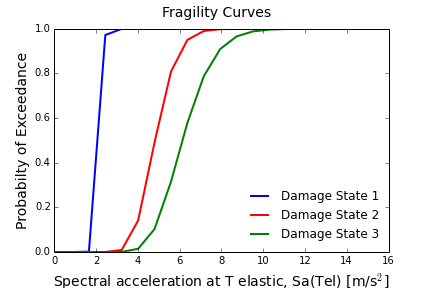
\includegraphics[width=12cm,height=8cm]{./figures/IdealisedCurve.png}
\caption{Display of input Idealised pushover curve.}
\label{fig:expIdealised}
\end{figure}

\begin{figure}[H]
\centering
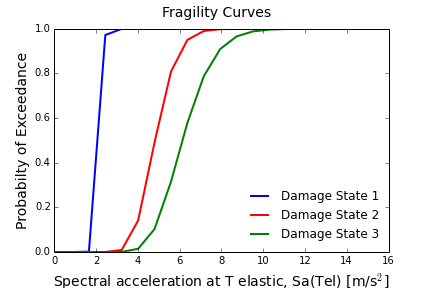
\includegraphics[width=12cm,height=8cm]{./figures/IdealisedCurve.png}
\caption{Display of input pushover curve.}
\label{fig:expPushover}
\end{figure}

In the third step of the code the fragility curves are derived. The simplified\_bilinear function makes use of the parameters extracted to derive ductility levels $\mu$, median Spectral accelerations $\hat{S}_{a,ds}(T_1)$ and the total dispersions $\beta_{sc}$ at each damage threshold, following the steps from 2 to 7 of Section ~\ref{subsec:CalculationSteps}. These results can be visualised during the analysis, as shown below. They are also exported in the folder output as cdv files and can be plotted if the variable plotflag[1] has been set to 1 (Figure ~\ref{fig:fragility}). These outputs are contained in the folder outputs, in the NSP directory.

\begin{Verbatim}[frame=single, commandchars=\\\{\}, samepage=true]
mu(LS) =  [ 0.73  1.87  2.55]
median IM =  [ 2.11  5.11  6.63]
total dispersion =  [ 0.09  0.32  0.46]
\end{Verbatim}

\begin{figure}[H]
\centering
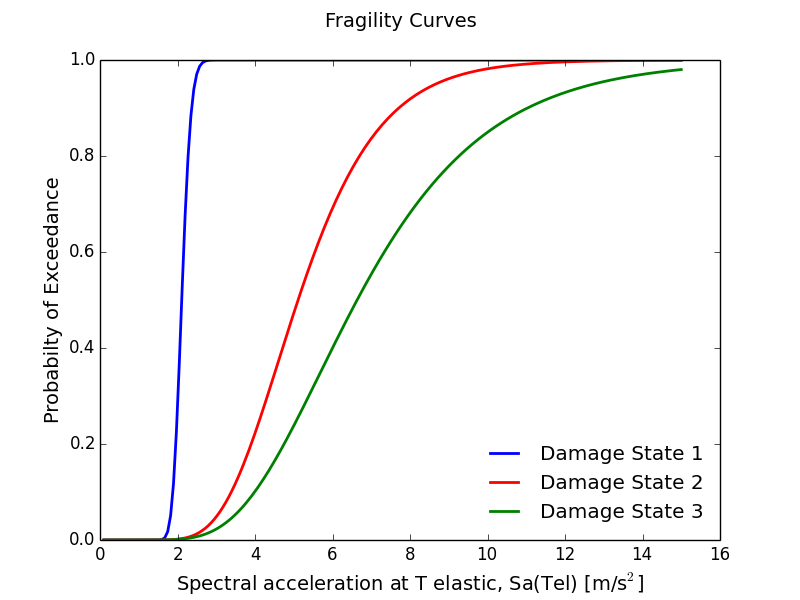
\includegraphics[width=12cm,height=8cm]{./figures/fragility.png}
\caption{Display of input pushover curve.}
\label{fig:fragility}
\end{figure}

If the variable vulnerability has been set to 1 a vulnerability curve is obtained in the fourth and final step. The derived fragility curves are used in conjunction with the consequence model selected as input, to get mean values and standard deviations of loss ratios at the intensity measure levels defined in the options (Section ~\ref{par:options}).
As in the case of the fragility curves the results are exported in csv format, and the plot is displayed and saved in png format if the variable plotflag[3] is set to 1. Both the csv and the png files can be found in the folder outputs in the NSP directory.

\subsubsection{Inter-building Uncertainty}
If the vulnerability curve wants to be derived for a class of buildings instead of for a single building the code is able to repeat the process for each single input-building and combine the outputs at the last stage of the results (fragility or vulnerability). 

The fragility results (converted into logarithmic mean and standard deviation of each Limit State) of each building are combined in four parameters: the mean and the standard deviations of the logarithmic means, and the mean and standard deviations of the logarithmic standard deviations. 

For the vulnerability curves instead a median loss ratio and the corresponding dispersion for each IML for each building are derived assuming a lognormal distribution. A Monte Carlo sampling is performed from these parameters to generate N loss ratios for each building for each IML, finally the mean and standard deviation of the sampled loss ratios is found. These parameters are converted into mean and coefficient of variation, which are the parameters consistent with Openquake input model.

In the input files the buildings to be analysed should be inserted as additional lines as in the example below:

\begin{table}[H]
\centering
\begin{tabular}{|c|c|c|} \hline
\textbf{n.building} & \textbf{T$_1$} & \textbf{$\Gamma_1$} \\ \hline
1 & 0.32 & 1.23\\ \hline
2 & 0.25 & 1.31\\ \hline
3 & 0.35 & 1.69\\ \hline
... & ... & ...\\ \hline
n & 0.41 & 1.54\\ \hline
\end{tabular}
\end{table}

\subsection{SPO2IDA based procedure}
Static PushOver to Incremental Dynamic Analysis (SPO2IDA) is a procedure originally developed by Vamvatsikos and Cornell (2006) and recommended in ATC-58 (FEMA P-58, 2012) that uses empirical relationships from a large database of incremental dynamic analysis results to convert static pushover curves into 16\%, 50\% and 84\% IDA curves. Given the idealised capacity curve the SPO2IDA tool uses an implicit R - $\mu$ - T relation to correlate nonlinear displacement, expressed in terms of ductility $\mu$ to the corresponding medians capacity in terms of spectral acceleration, $\hat{S}_{a,ds}(T_1) $). These medians capacity are defined as the values at which a given damage threshold has been attained or overcome by 50\% of the analysis conducted with the ground motion pairs. 

The record-to-record dispersion ??D is estimated by considering the number of records that have been used in the SPO2IDA spreadsheet ( ??D is estimated based on a large empirical database of incremental dynamic analysis results).

\subsection{Options}
Options (input: pushover-idealised curve, analysis: Ruiz-Garcia Miranda-Vamvatsikos and Cornell, vulnerability, uncertainty)

\subsection{Workflows}

Propagation of uncertainties
Outputs

\section{Nonlinear Dynamic Method for a class of buildings}
